% coding:utf-8

%FOSALRS, a LaTeX-Code for a electrical summary of control theory
%Copyright (C) 2013, Daniel Winz, Ervin Mazlagic

%This program is free software; you can redistribute it and/or
%modify it under the terms of the GNU General Public License
%as published by the Free Software Foundation; either version 2
%of the License, or (at your option) any later version.

%This program is distributed in the hope that it will be useful,
%but WITHOUT ANY WARRANTY; without even the implied warranty of
%MERCHANTABILITY or FITNESS FOR A PARTICULAR PURPOSE.  See the
%GNU General Public License for more details.
%----------------------------------------

\section{Einstellregeln PID Regler}

\subsection{Ziegler-Nichols}
Die Regelstrecke wird als $PT_1$ Glied mit Totzeit betrachtet. 
\[ G_S(s) = \frac{K_S \cdot e^{-T_t}}{1 + s \cdot T_S} \]

\subsubsection{Übergangsmethode}
\[
    \begin{array}{lccc}
        &
            K_R &
            T_N &
            T_V \\\\
        \text{P} &
            \frac{T_S}{K_S \cdot T_t} &
            - &
            - \\\\
        \text{PI} &
            \frac{0.9 \cdot T_S}{K_S \cdot T_t} &
            3.3 \cdot T_t &
            - \\\\
        \text{PID} &
            \frac{1.2 \cdot T_S}{K_S \cdot T_t} &
            2.0 \cdot T_t &
            0.5 \cdot T_t \\\\
    \end{array}
\]

\subsubsection{Stabilitätsgrenzenmethode}
$K_R$ wird erhöht, bis eine Schwingung auftritt. $\to K_R = K_{krit}$\\
Dabei wird die Schwingtauer $T_{krit}$ bestimmt. \\\\
Alternativ können $K_{krit}$ und $T_{krit}$ auch aus dem Bodediagramm oder 
aus der Nyquist Ortskurve gelesen werden. $T_{krit} = \frac{2 \pi}{\omega_{krit}}$
\[
    \begin{array}{lccc}
        &
            K_R &
            T_N &
            T_V \\\\
        \text{P} &
            0.5 \cdot K_{krit} &
            - &
            - \\\\
        \text{PI} &
            0.45 \cdot K_{krit} &
            0.83 \cdot T_{krit} &
            - \\\\
        \text{PID} &
            0.6 \cdot K_{krit} &
            0.5 \cdot T_{krit} &
            0.125 \cdot T_{krit} \\\\
    \end{array}
\]


\subsection{Chien, Hrones und Reswick}
Regelstrecken mit Verzögerung und ohne Überschwingen
\begin{figure}[h!]
    \centering
    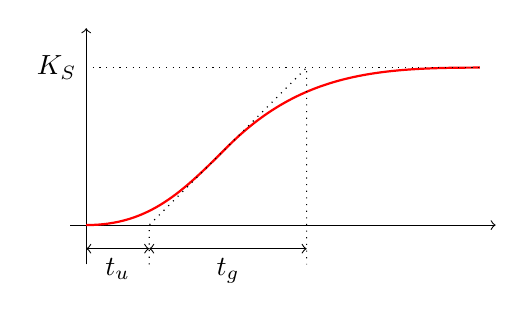
\begin{tikzpicture}
        \draw[->] (-0.2,0) -- (5.2,0);
        \draw[->] (0,-0.5) -- (0,2.5);
        \draw[red, thick] (0,0) to[out=0, in=225] (1.8,1) to[out=45, in=180] (5,2);
        \draw[dotted] (0,2) node[left] {$K_S$} -- (5,2);
        \draw[dotted] (0.8,-0.5) -- (0.8,0) -- (2.8,2) -- (2.8,-0.5);
        \draw[<->] (0,-0.3)   -- node[below] {$t_u$} (0.8,-0.3);
        \draw[<->] (0.8,-0.3) -- node[below] {$t_g$} (2.8,-0.3);
    \end{tikzpicture}
\end{figure}
\\
\begin{tabular}{@{}ll}
    $K_s$: & Streckenverstärkung\\
    $t_u$: & Verzugszeit\\
    $t_g$: & Ausgleichszeit\\
\end{tabular}

\subsubsection{Optimierung des Störverhaltens, Aperiodischer Regelverlauf}
\[
    \begin{array}{lccc}
        &
            K_R &
            T_N &
            T_V \\\\
        \text{P} &
            0.3 \cdot \frac{t_g}{t_u \cdot K_S} &
            - &
            - \\\\
        \text{PI} &
            0.6 \cdot \frac{t_g}{t_u \cdot K_S} &
            4.0 \cdot t_u &
            - \\\\
        \text{PID} &
            0.95 \cdot \frac{t_g}{t_u \cdot K_S} &
            2.4 \cdot t_u &
            0.42 \cdot t_u \\\\
    \end{array}
\]

\subsubsection{Optimierung des Störverhaltens, 20\% Überschwingen}
\[
    \begin{array}{lccc}
        &
            K_R &
            T_N &
            T_V \\\\
        \text{P} &
            0.7 \cdot \frac{t_g}{t_u \cdot K_S} &
            - &
            - \\\\
        \text{PI} &
            0.7 \cdot \frac{t_g}{t_u \cdot K_S} &
            2.3 \cdot t_u &
            - \\\\
        \text{PID} &
            1.2 \cdot \frac{t_g}{t_u \cdot K_S} &
            2.0 \cdot t_u &
            0.42 \cdot t_u \\\\
    \end{array}
\]

\subsubsection{Optimierung des Führungsverhaltens, Aperiodischer Regelverlauf}
\[
    \begin{array}{lccc}
        &
            K_R &
            T_N &
            T_V \\\\
        \text{P} &
            0.3 \cdot \frac{t_g}{t_u \cdot K_S} &
            - &
            - \\\\
        \text{PI} &
            0.35 \cdot \frac{t_g}{t_u \cdot K_S} &
            1.2 \cdot t_g &
            - \\\\
        \text{PID} &
            0.6 \cdot \frac{t_g}{t_u \cdot K_S} &
            1.0 \cdot t_g &
            0.5 \cdot t_u \\\\
    \end{array}
\]

\subsubsection{Optimierung des Führungsverhaltens, 20\% Überschwingen}
\[
    \begin{array}{lccc}
        &
            K_R &
            T_N &
            T_V \\\\
        \text{P} &
            0.7 \cdot \frac{t_g}{t_u \cdot K_S} &
            - &
            - \\\\
        \text{PI} &
            0.6 \cdot \frac{t_g}{t_u \cdot K_S} &
            1.0 \cdot t_g &
            - \\\\
        \text{PID} &
            0.95 \cdot \frac{t_g}{t_u \cdot K_S} &
            1.35 \cdot t_g &
            0.47 \cdot t_u \\\\
    \end{array}
\]

\subsection{Aström}


